\chapter{Gravity Inversion}\label{Chp:cook:gravity inversion}

\section{Introduction}

In this part the documentation we give an introduction on how to us the \downunder module using the 
inversion driver functions to perform the inversion of gravity and magnetic data. The driver functions 
enables geologists and geophysicists apply the \downunder module quickly and in easy way
with out a detailed knowledge of the theory of inversion or programming skills. However, users
how are interested in specializing or extending the inversion capacity are referred to the second part~\ref{part2}
of this manual. It is beyond the intention of this manual to give a in-detailed introduction to
geophysical inversion in particular to the appropriate preprocessing of data sets. We refer to~\cite{REF1, REF2, REF3}.


The \downunder function described here are designed for calculate estimations for the 
3-D distribution of density and/or susceptibility from 2-D gravity and magnetic data measured in ground 
or airborne surveys. This process is generally called inversion of geophysical data.
Following the standard assumption it is assumed that the 
data are measured as perturbation of an expected gravity and/or magnetic
field of the Earth. In this context measured gravity and magnetic data are in fact describing anomalies in 
gravity and magnetic field. As a consequence the inversion process 
provides corrections to an average density (typically $2670 kg/m^3$) and susceptibility (typically $0$). 
So in the following we will always assume that given data for anomalies are given and therefore
not in all cases explicitly use the terms such gravity anomalies or density corrections but just use the terms
gravity and density.

In this chapter we will give a detailed introduction into usage of the driver functions 
for inversion of gravity data. In the following chapters~\ref{Chp:cook:magnetic inversion} and~\ref{Chp:cook:joint inversion}
we will discuss the inversion of magnetic and the joint inversion of gravity and magnetic data using 
\downunder. As the same principles as for gravity data apply the presentation for these problem classes is kept short and 
users interested in magnetic data only should still work through this chapter on gravity data. 

To run the examples discussed you need to have \escript (version 3.3.1 or newer) installed on your computer.
Moreover, if you want to visualize result, you must have access to plotting software which is able to process
\VTK input files, e.g. \mayavi and \VisIt. As \mayavi can easily be obtained and installed for most platforms
the tutorial is based on \mayavi as visualization. However, it pointed out 
that \VisIt is the preferred visualization tool for \escript as it can deal with very large data sets more effectively.
    
\begin{figure}
\centering
\includegraphics[width=0.7\textwidth]{QLDWestGravityDataPlot.png}
\caption{Gravity Anomaly Data in $mgal$ from Western Queensland, Australia, see file \examplefile{data/QLDWest_grav.nc}.
 \AZADEH{ADD CREDITS}}
\label{FIG:P1:GRAV:0}
\end{figure}

\begin{figure}
\centering
\includegraphics[width=0.7\textwidth]{QLDGravMu10Contour.png}
\caption{3D contour plot of density distribution of inversion of data \file{data/QLDWest_grav.nc} ($\mu=10$). Colors
represent values of density where high values are represented by red and low values are represented by blue.
 \AZADEH{mu=10?}}
\label{FIG:P1:GRAV:1}
\end{figure}

\section{How does it work?}
The execution of the inversion is controlled by script which is in essence is a text file. This can be edited using any 
text editor. The script contains a serious of statements which are executed from an interpreter which
is an executable program reading the text file and executing the statements line-by-line. In the case 
of \downunder the interpreter is \python. In order to be able to process the statements in each line of the script
certain rules (called syntax) need to be obeyed. There is large number of online tutorials for \python 
available\footnote{e.g. \url{http://www.tutorialspoint.com/python} and \url{http://doc.pyschools.com}}. We also 
refer to the \escript cook book \cite{ESCRIPTCOOKBOOK} and users guide \cite{ESCRIPT} which is in particular useful for users which who to dive deeper
\downunder. For this part of the manual no \python knowledge is required but it is recommended that 
users acquire some basic knowledge on \python as they progressing in their work with \downunder.

The following script~\ref{code: garvity1}\footnote{The script is similar to the \examplefile{grav_netcdf.py} script
find in the \escript example file directory.} is a simple example to run an inversion for gravity data: 
\begin{pyc}
\
\begin{verbatim*}
# Header:
from esys.downunder import *
from esys.weipa import *
import esys.escript.unitsSI as U

# Step 1: set up domain
dom=DomainBuilder()
dom.setVerticalExtents(depth= 40.*U.km, air_layer=6.*U.km, num_cells=25)
dom.setFractionalPadding(pad_x=0.2, pad_y=0.2)
dom.fixDensityBelow(depth= 40. * U.km)

# Step 2: read gravity data
source0=NetCdfData(NetCdfData.GRAVITY, 'data/QLDWest_grav.nc',altitude=0.)
dom.addSource(source0)

# Step 3: set up inversion
inv=GravityInversion()
inv.setSolverTolerance(1e-4)
inv.setSolverMaxIterations(50)
inv.setup(dom)

# Step 4: run inversion 
inv.getCostFunction().setTradeOffFactorsModels(10.) 
rho = inv.run()

# Step 5: write reconstructed density to file
saveVTK("result.vtk", density=rho)
\end{verbatim*}\label{code: garvity1}
\end{pyc}
The result, in this
case the density distribution, is written to an internal file for further processing. You can copy and past the text of the 
script into a file of any name, let's say for further reference we use the file name \file{grav.py}. It is recommendable
to use the extention \file{py} to identify the file as \python script. We will discuss the statements
of the script later in this chapter. 

Obviously the inversion needs to be fed with some gravity data. In this case 
the data are loaded from the file \examplefile{data/QLDWest_grav.nc} which available in the \escript example file directory. The data are given 
in the \netcdf data format for gridded data. After you have copied this file into the directory in which you have
saved the script \file{grav.py} you can run the program using the command line 
\begin{verbatim}
run-escript grav.py
\end{verbatim}
We are running \file{grav.py} through the \escript start-up command as \escript is used as a back end for the inversion 
algorithm\footnote{Please see the \escript users guide~\cite{ESCRIPT} on how to run 
your script in parallel using threading and/or MPI.}. Obviously it is  assumed that you have an
installation of \escript available on your computer, see \url{https://launchpad.net/escript-finley}.

After the execution has successfully been completed you will find the result file \file{result.vtk} in the directory
from where you have started the execution of the script. the file is using the \VTK format and can be important 
easily into many visualization tools. One option is the \mayavi package which is available on most platforms. You can invoke the
the visualization using the commands
\begin{verbatim}
mayavi2 -d result.vtu -m SurfaceMap
\end{verbatim}
from the command line. Figure~\ref{FIG:P1:GRAV:1} shows the result using contour plotting\footnote{Plots
have been created with \VisIt.} from the gravity anomaly data shown in Figure~\ref{FIG:P1:GRAV:0}. We will 
discuss data later in Section~\ref{SEC:P1:GRAV:DATA}.

Let us have a closer look at the script\footnote{In \python lines starting with `\#` are commends and are not processed further.}: Besides the header section one can separate the script into five steps:
\begin{enumerate}
 \item set up domain on which the inversion problem is solved
 \item load the data 
\item set-up the inversion problem
\item run the inversion
\item further processing of the result, here we write the reconstructed density distribution to a file.
\end{enumerate}
In the following we will discuss the steps of the scripts in more details. Before we do this it is pointed out that
the header section which, by following \python standards, makes all the package we need available to access within the script. At this
point we will not discuss this in more details but emphasize that the header section is a vital part of the script. It is is required 
in each \downunder inversion script and should not be altered accept if additional modules are needed. 

\begin{figure}
\centering
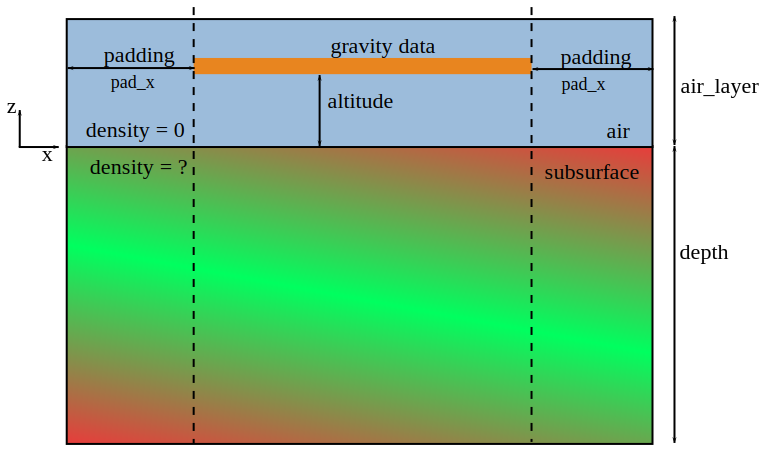
\includegraphics[width=\textwidth]{dom2D.png}
\caption{2D domain set-up for gravity inversion.}
\label{FIG:P1:GRAV:2}
\end{figure}

\section{How to create the inversion Domain}
First step in the script~\ref{code: garvity1} is the definition of the domain over which the inversion is performed.
We think of the domain as a block with orthogonal, plain faces. Figure~\ref{FIG:P1:GRAV:2} shows the set-up for 
a two dimensional domain (see also Figure~\ref{fig:domainBuilder} for 3D). The lateral coordinates along the 
surface of the Earth are denoted by $x$ and $y$ (on $x$-direction is shown). The $z$ direction defines the
vertical direction where the part above the surface has positive coordinates and the 
subsurface negative coordinates. The height of the section above the surface which is assumed to be filled to with air 
needs to be set by the user. The inversion assumes that the density in the section is known to be zero. The density
below the surface is unknown and is calculated through the inversion. The user needs to specify the depth below
the surface in which the density is to be calculated. 
The lateral extension of the domain is defined by the data sets fed into the inversion. It is chosen large enough
to cover all data sets. In order to reduce the impact of boundary a padding zone around the data sets can be introduced.
  
\begin{figure}
\centering
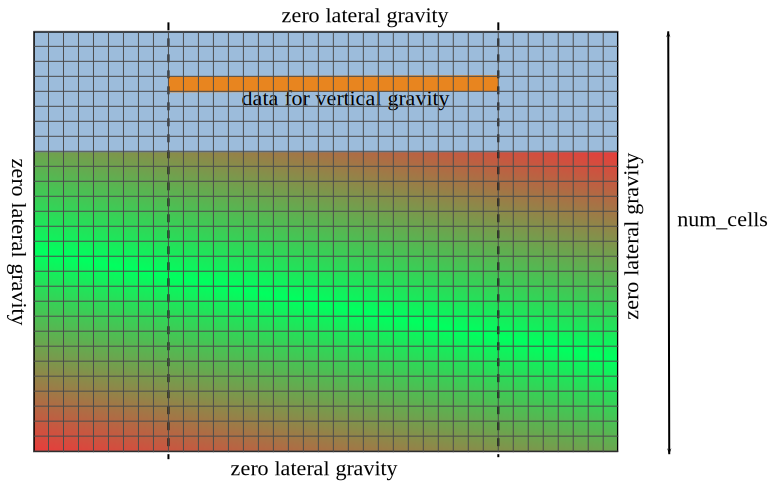
\includegraphics[width=\textwidth]{dom2DFEM.png}
\caption{Cell distribution and boundary conditions for 2D domain.}
\label{FIG:P1:GRAV:3}
\end{figure}

The reconstruction of the gravity field from an estimated density distribution is a the key component of the inversion process.
To do this \downunder uses the finite element method (FEM) to do this. We need to introduce a grid over the domain, see Figure~\ref{FIG:P1:GRAV:3}.
The number of vertical cells is set by the user while the number of vertical cells is derived from the grid spacing of the 
gravity data set(s). It is assumed that gravity field data given are constant across a cell. 
To be able to reconstruct the gravity field some assumptions on the values of the gravity field on the domain boundary
have to made. \downunder assumes that on all faces the lateral gravity field component equals 
zero. No assumptions on the 
horizontal components are made\footnote{It is assumed that the gravity potential equals zero on the top and bottom
surface, see Section~\ref{sec:forward gravity} for details}\footnote{Most inversion codes are using Green's function over an unbounded domain to reconstruct the gravity field. This approach
makes the assumption the gravity field (or potential) is converging to zero when moving away from the region of interest. The 
boundary conditions used here are stronger in the sense that the lateral gravity component is enforced to zero in 
a defined distance of the region of interest but weaker in the sense that no constraint on the horizontal component is applied.}.
   
In script~\ref{code: garvity1} the statement
\begin{verbatim}
dom=DomainBuilder()
\end{verbatim}
creates same form of a factory to build a domain. 
We define the features of the domain we would like to create:
\begin{verbatim}
dom.setVerticalExtents(depth= 40.*U.km, air_layer=6.*U.km, num_cells=25)
dom.setFractionalPadding(pad_x=0.2, pad_y=0.2)
\end{verbatim}
Here we define the depth of the domain to $40 km$, the thickness of the air layer above the surface to $6km$ and 
the number of vertical cells to $25$. We also introduce a lateral padding of $20 \%$ of the expansion of
the gravity data on each side of the data and in both lateral directions.

In some cases it can be appropriate to assume that the density below a certain depth is 
zero\footnote{As we are in fact calculate density corrections this means that the density is assumed to be
the average density.}. The statement 
\begin{verbatim}
dom.fixDensityBelow(depth= 40. * U.km)
\end{verbatim}
introduces this constrain. As in the case discussed here the depth for zero density is not less than the
depth of the domain no constraint at depth is applied to the density.

\downunder uses the  metre-kilogram-second based 
International System of Units (SI)~\footnote{see \url{http://en.wikipedia.org/wiki/International_System_of_Units}.}\index{SI}. So all 
values must be converted to appropriate units. This does not apply to geographic coordinates where \downunder uses
the degree with fractional degree (as a floating number) to represent longitude and latitude. In the script we have used the expression
\begin{verbatim}
depth= 40. * U.km
\end{verbatim}
to define the depth of the domain to $40 km$. The expression \verb|U.km| is the unit $km$ (kilo meter) and an appropriate conversion 
of $40$ as length in $km$  into the base unit $m$ (meter). It is recommendable to add units to values (where present) 
in order to make sure that the final value handed into \downunder is given in the appropriate units. The physical units
module of \escript, which we have here imported under the name \verb|U| in the script header, defines a large number 
physical units and constants, please see~\cite{ESCRIPT} and~\cite{ESCRIPTONLINE}. 

\section{How to Load Gravitational Data}\label{SEC:P1:GRAV:DATA}
In practice gravity acceleration is measured in various way, for instance by airborne surveys~\cite{Telford1990a}. \downunder
assumes that at input that appropriate processing has been applied,  
in particular, corrections for  
\begin{itemize}
 \item free-air to remove effects from altitude above ground 
 \item latitude to remove effects from ellipsoidicity of the Earth  
 \item terrain to remove effects from topography  
\end{itemize}
have been applied to the data. In general, data prepared in such a form are called Bouguer anomalies~\cite{Telford1990a}. 

To load gravity data into  \downunder the data are given on a plane parallel to the surface of the Earth at a constant
altitude, see diagram~\ref{FIG:P1:GRAV:2}. The data need to be defined over a rectangular grid covering a subregion of 
the Earth surface. 
The grid is using the geographic coordinate system. Figure~\ref{FIG:P1:GRAV:0} shows an example of such a data set
from the westen parts of Queensland. The data set covers a rectangular region between $140^o$ and $141^o$ east 
and between $20^o$ and $21^o$ south. Notice that latitude varies between $-90^o$ to $90^o$ where
negative signs refer to places in the southern hemisphere and
longitude varies between $-180^o$ to $180^o$ where
negative signs refer to places in the western hemisphere.
The color at a location represent the value of the vertical Bouguer gravity in  anomaly at this point at the surface of the Earth.
Values range from $-160  \;  mgal$ to about $500 \; mgal$\footnote{$mgal$ refers to milli $gal$ (galileo) with 
$1 \;  gal = 0.01 \frac{m}{sec^2}$.} over $121 \times 121$ grid.

In general, a patch gravity data need to be defined over a plane \verb|NX| $\times$ \verb|NY| where 
\verb|NX|  and \verb|NY|  define the number of grid lines in the longitude (\verb|X|) and the latitude (\verb|Y|) 
direction, respectively. The grid is spanned of from an origin with spacing
\verb|DELTA_X| and \verb|DELTA_Y| in the longitude and the latitude direction, respectively. 
The gravity data for all grid points need to be given as an \verb|NX| $\times$ \verb|NY| array.  
If available errors can be associated with the gravity data. The values are given as an \verb|NX| $\times$ \verb|NY| array
matching the shape of the gravity. 
The \python script \examplefile{create_netcdf.py} shows how to create a file in the \netcdf file format~\cite{NETCDF}.
see Section~\ref{SEC:P1:GRAV:REMARK:DATAHOLES}
BLA 

\CIHAN{ADD an example how ro use ER Mapper raster files}

In addition to the \netcdf file format 


Two data formats are supported, namely ER Mapper Raster File and NetCDF. Here we will
focus on the NetCDF file format~\cite{NETCDF} and refer to subsection~\ref{SEC:P1:GRAV:REMARK:ERMAPPER} and
section~\ref{sec:ref:DataSource:ERM} for more information on the ER Mapper Raster format.

BLA
In script~\ref{code: garvity1} we use the statement 
\begin{verbatim}
source0=NetCdfData(NetCdfData.GRAVITY, 'data/QLDWest_grav.nc',altitude=0.)
\end{verbatim}
\CIHAN{REWISE} \AZADEH{ADD coarse data 10x10 or so?} 
to load the gravity data stored in \examplefile{data/QLDWest_grav.nc} in the \netcdf format. 
Within the script The data set is now available under the name \verb|source0|. We need to link
the data set to the \verb|DomainBuilder| using 
\begin{verbatim}
dom.addSource(source0)
\end{verbatim}
At the time the domain for the inversion is build the \verb|DomainBuilder| will use the information about
origin, extension and spacing along with the other options provided to build an appropriate domain. As at this point a
flat Earth is assumed geographic coordinates used to represent data in the input file 
are mapped to a (local) Cartesian coordinate system is applied. By default \CIHAN{WHAT} is used. 
This transformation can be overwritten    \CIHAN{YES? HOW?}   
   
It is possible to added several, possibly overlapping data sets to the same domain:
\begin{verbatim}
source0=NetCdfData(NetCdfData.GRAVITY, 'data0.nc',altitude=0.)
source1=NetCdfData(NetCdfData.GRAVITY, 'data1.nc',altitude=0.)
dom.addSource(source0)
dom.addSource(source1)
\end{verbatim}
\CIHAN{Restrictions? Same Zone? Grid alignment?}

It is important to keep an eye of the complexity of the inversion. A good measure is the total number of cells 
being used. Assume we have given a data set on $20 \times 20$ grid. As lateral padding is added, lets say 
we add $20 \%$ to each side of the data, the lateral number of cells is given as $(20 \cdot 1.4) \times (20 \cdot 1.4)$
which given a value of $1.4^2 \cdot 20^2 \approx 2 \cdot 10^2 = 800$. If we use $20$ cells in vertical direction
we end up with a total number of $800 \times 20 = 16,000$ cells. This size can easily be handed by a desk top PC.
If we increase the grid size of the data to $40 \times 40$ grid and
use $40$ cells in the vertical extend we get a total number of $( 2 \cdot 40^2) \cdot 50 =128,000$ a problem size
which can still be handled by a desk top computer. If the grid of the data is increased 
to $200 \times 200$ and we use $200$ cells in the vertical extend the domain will contain $16,000,000$ ($16$ million cells). 
It will require a bigger computer to run the inversion. This estimate of complexity growth applies to the case where the increase 
of data grid size is driven by an increase of resolution where it is recommendable to increase the 
vertical resolution in sink with the lateral resolution. In other cases the expansion of the region of
interest drives an increase of data grid size the increase of total number of cells is less dramatic as
the vertical number of cells can remain constant while keeping a balanced resolution in vertical and lateral direction.


\section{Set-up Inversion and Run It}
We are now at step three of script~\ref{code: garvity1} in which the actual inversion is set-up. First 
we create an empty inversion under the name \verb|inv|:
\begin{verbatim}
inv=GravityInversion()
\end{verbatim}
As indicated by the name we create an inversion of gravity 
data\footnote{\verb|GravityInversion| is driver with a simplified interface 
which is provided for convenience. See Part~\ref{part2} for more details 
on how to write inversion scripts with more general functionality, e.g. constraints.}. The inversion
is an iterative process which sequentially calculates updates to the density distribution 
in the attempt to improve the match of the gravity field produced by the density distribution with the data. 
Termination of the iteration is controlled by the tolerance to be set by the user:
\begin{verbatim}
inv.setSolverTolerance(1e-4)
\end{verbatim}
Here we set the tolerance to $10^{-4}$, i.e. the iteration is terminated if the maximum density correction
is less or equal to $10^{-4}$ relative to the maximum value of estimated density anomaly. In case the 
iteration is not converging a maximum number of iteration step is set:  
\begin{verbatim}
inv.setSolverMaxIterations(50)
\end{verbatim}
If the maximum number iteration steps (here $50$ steps) is reached the iteration is aborted and an error message is
printed. In the case you can try to rerun the inversion with a larger value for the maximum number iteration steps. If even for 
a very large number of iteration steps no convergence is observed, this is a strong indicator that the inversion has not been
set up properly. 

The statement 
\begin{verbatim}
inv.setup(dom)
\end{verbatim}
links the inversion with the domain and the data. At this step - as we are solving a gravity inversion problem -
only gravitational data attached to the domain \verb|dom| are considered. Internally a cost function $J$
is created which is minimized during the inversion iteration. It is a combination of
a measure of the data misfit of the gravity field from the given density distribution and 
a measure of the smoothness of the density distribution. The latter is often called the regularization term. By default 
the gradient of density is used as the regularization term, see also section~\ref{SEC:P1:GRAV:REMARK:REG}. 
Obviously, the result of the inversion is sensitive to the weighting between the misfit and the regularization. This
trade-off factor $\mu$ for the misfit function is set by the following statement:
\begin{verbatim}
inv.getCostFunction().setTradeOffFactorsModels(0.1) 
\end{verbatim}
Here we set $\mu=0.1$. The statement \verb|inv.setup| must appear in the script before setting of the trade-off factor.
A small value for the trade-off factor $\mu$ will give more emphasize to the regularization component 
and create a smoother density distribution. A large value the trade-off factor $\mu$ will put more emphasize on the
misfit and typically create a better fit to the data and a rougher density distribution. It is important to keep in mind that
the regularization reduces noise in the date and in fact gives the problem a unique solution. Consequently 
the trade-off factor $\mu$ may not be chosen too large in order control the noise on the solution and ensure convergence in
the iteration process.

We can now actually run the inversion:
\begin{verbatim}
rho = inv.run()
\end{verbatim}
The answer as calculated during the inversion is returned and can be accessed under the name \verb|rho|. As pointed out earlier
the iteration process may fail in which case the execution of the script is aborted. 

\section{Take a look}
In the final step of script~\ref{code: garvity1} the calculated density distribution is written to an external file. 
A file format which is used by several visualization packages such as \VisIt~\cite{VISIT} and \mayavi~\cite{MAYAVI}
is the \VTK file format. The result of the inversion which has been named \verb|rho| can be written to the file 
\file{result.vtu} by adding the statement
\begin{verbatim}
saveVTK("result.vtu", density=rho)
\end{verbatim}
to the end of script. It is recommendable to use the extension \verb|vtu| for the \VTK result files. 
The inversion solution is tagged with name \verb|density| in the result file. Notice that any other
name for the tag could be used. As the format is text based
\VTK files tend to be very large and take compute time to create in particular when it comes to large numbers of cells ($>10^6$).
For large problems it is more efficient to use the \SILO file format~\cite{SILO}. \SILO files tend to be smaller 
and to be faster generated and read. It is the preferred format to import results into the visualization program \VisIt~\cite{VISIT}
which is particularly suitable for the visualization of large data sets. Inversion results can directly exported into \SILO files using
the statement:       
\begin{verbatim}
saveSilo("result.silo", density=rho)
\end{verbatim}
replacing the \verb|saveVTK| statement. Similarly, to \VTK files the result \verb|rho| is tagged 
with the name \verb|density| so it can be identified in the visualization program. 

\begin{figure}
	     \begin{center}
        \subfigure[$\mu=0.1$]{%
	            \label{FIG:P1:GRAV:10 MU01}
	            \includegraphics[width=0.45\textwidth]{QLDGravMu01Contour.png}
	        }%
	        \subfigure[$\mu=1.$]{%
	           \label{FIG:P1:GRAV:10 MU1}
	           \includegraphics[width=0.45\textwidth]{QLDGravMu1Contour.png}
	        }\\ %  ------- End of the first row ----------------------%
	        \subfigure[$\mu=10.$]{%
	            \label{FIG:P1:GRAV:10 MU10}
	            \includegraphics[width=0.45\textwidth]{QLDGravMu10Contour.png}
	        }%
	        \subfigure[$\mu=100.$]{%
	            \label{FIG:P1:GRAV:10 MU100}
	            \includegraphics[width=0.45\textwidth]{QLDGravMu100Contour.png}
	        }%
	%
	    \end{center}
	   \label{FIG:P1:GRAV:10}

\caption{3D Contour plots of gravity inversion with gravity data from Figure~\ref{FIG:P1:GRAV:0} for
various values for model trade-ff factor $\mu$. Visualization has been performed \VisIt. \AZADEH{check images.}}
\end{figure}

\begin{figure}
	     \begin{center}
        \subfigure[$\mu=0.1$]{%
	            \label{FIG:P1:GRAV:11 MU01}
	            \includegraphics[width=0.45\textwidth]{QLDGravMu01Slice.png}
	        }%
	        \subfigure[$\mu=1.$]{%
	           \label{FIG:P1:GRAV:11 MU1}
	           \includegraphics[width=0.45\textwidth]{QLDGravMu1Slice.png}
	        }\\ %  ------- End of the first row ----------------------%
	        \subfigure[$\mu=10.$]{%
	            \label{FIG:P1:GRAV:11 MU10}
	            \includegraphics[width=0.45\textwidth]{QLDGravMu10Slice.png}
	        }%
	        \subfigure[$\mu=100.$]{%
	            \label{FIG:P1:GRAV:11 MU100}
	            \includegraphics[width=0.45\textwidth]{QLDGravMu100Slice.png}
	        }%
	%
	    \end{center}
	   \label{FIG:P1:GRAV:11}

\caption{3D Slicing plots of gravity inversion with gravity data from Figure~\ref{FIG:P1:GRAV:0} for
various values for model trade-ff factor $\mu$. Visualization has been performed \VisIt. \AZADEH{check images.}}
\end{figure}

Figures~\ref{FIG:P1:GRAV:10} and~\ref{FIG:P1:GRAV:11} show two different styles of visualization performed by \VisIt
on the result of the inversion of the gravity anomalies shown in Figure~\ref{FIG:P1:GRAV:0}. The inversions
have been performed with different values for the  model trade-off factor $\mu$. The visualization shows 
clearly the smoothing effect of lower values for the trade-off factors. For larger values of the trade-off factor
the density distribution becomes rougher showing larger details. Computational costs are significantly higher 
for larger trade-off factors. Moreover, noise in the data has an higher impact on the result. Typically several 
runs are required to adjust the value for the trade-off factor.


For some analysis tools it is useful to process the results in form of Comma Separated Values (\CSV)~\footnote{see 
\url{http://en.wikipedia.org/wiki/Comma-separated_values}.}. Such a file can be created using the statement
\begin{verbatim}
saveCSV("result.csv", x=rho.getFunctionSpace().getX(), density=rho)
\end{verbatim}
in the script. This will create a \file{result.csv} with columns separated by comma. Each row contains the value of the
density distribution and the three coordinates of the corresponding location in the domain. There is a header specifying 
the meaning of the corresponding column. \LG{Add example output CSV}. Notice that rows are not written in a particular 
order and therefore, if necessary, the user has to apply appropriate sorting to the rows.
Columns are written in alphabetic order of their corresponding tag names. For the interested reader: The 
statement \verb|rho.getFunctionSpace()| returns the type used to store the density data \verb|rho|.
The  \verb|getX()| returns the coordinates of the sampling points used for the particular type of
representation, see~\cite{ESCRIPT} for details. 


\section{Remarks}

\subsection{Data With Holes}\label{SEC:P1:GRAV:REMARK:DATAHOLES}
\CIHAN{ADD some remarkes hol;es in the data, example?}


\subsection{ER Mapper Raster File}\label{SEC:P1:GRAV:REMARK:ERMAPPER}
\CIHAN{ADD an example how ro use ER Mapper raster files}

\subsection{Regularization Term}\label{SEC:P1:GRAV:REMARK:REG}
\verb|GravityInversion| supports the following form for the regularization:
\begin{equation}
\int w^{(0)} \cdot \rho^2 + w^{(1)}_0  \rho_{,0}^2 +  w^{(1)}_1  \rho_{,1}^2 +  w^{(1)}_2  \rho_{,2}^2\; dx   
\end{equation}
where the integral is calculated across the entire domain. $\rho$ represents the density distribution 
where $\rho_{,0}$ $\rho_{,1}$ and $\rho_{,2}$ are the spatial derivatives of $\rho$ with respect to the 
two lateral and the vertical direction, respectively.  
$w^{(0)}$, $w^{(1)}_0$, $w^{(1)}_1$ and $w^{(1)}_2$ are weighting factors\footnote{A more general form, e.g. spatially variable values
for the weighting factors, is supported, see Part~\ref{part2}}. By default it set
$w^{(0)}=0$, $w^{(1)}_0=w^{(1)}_1=w^{(1)}_2=1$. Other weighting factors can be set in the inversion set-up. For instance to
set $w^{(0)}=10$,
$w^{(1)}_0=w^{(1)}_1=0$ and $w^{(1)}_2=100$ use the statement:
\begin{verbatim}
inv.setup(dom, w0=10, w1=[0,0,100])
\end{verbatim}
It is pointed out that the weighting factors are rescaled in order improve numerical stability. Therefore the relative size of
the weighting factors is relevant and using  
\begin{verbatim}
inv.setup(dom, w0=0.1, w1=[0,0,1])
\end{verbatim}
would lead to the same regularization like the statement above.


% 
% \section{Reference}
% 
% There are three examples for 2D and 3D gravity inversions with artificial input data.
% In first step, an area with synthetic density section was suggested. Then based on forward modeling its gravitational data was collected. Afterwards with generated gravity data, escripts simulated a volume of inverted density. Whilst new density mass could be compared with the synthetic density section to verify the inversion.
% 
% Some of the presumptions were the same for all of the examples to simplify the situation to make a logical comparison between synthetic input and output. which is as followed:
% 
% \begin{verbatim}
% n_cells_in_data=100
% depth_offset=0.*U.km
% l_data = 100 * U.km
% l_pad=40*U.km
% THICKNESS=20.*U.km
% l_air=6*U.km
% \end{verbatim}
% 
% The others assumptions comes with each examples.
% \begin{enumerate}
% \item  A 2D density section with a maximum in center was assumed. The reference density and inverted will be shown. The padding area is excluded. (\ref{fig:gravity2D1})
% 
% \begin{verbatim}
% n_cells_in_data=100
% n_humbs_h= 1
% n_humbs_v=1
% mu=100
% \end{verbatim}
% 
% \begin{figure}
% \centering
% \includegraphics[width=\textwidth]{grav2D1.png}
% \caption{2D density model up) reference    down) result}
% \label{fig:gravity2D1}
% \end{figure}
% 
% 
% \item A 2D density properties with two maximum in corners and one minimum in the center was inverted. The result have eliminated the effects in padding area.(\ref{fig:gravity2D3}) 
% 
% \begin{verbatim}
% n_cells_in_data=100
% n_humbs_h= 3
% n_humbs_v=1
% mu=100
% \end{verbatim}
% 
% \begin{figure}
% \centering
% \includegraphics[width=\textwidth]{grav2D3.png}
% \caption{2D density model up) reference  down) result}
% \label{fig:gravity2D3}
% \end{figure}
% 
% \item A 3D model with a maximum in the center was used as input data and the result after simulation in shown in the next image which determined a good distribution of density through the model in the main area.(\ref{fig:gravity3D} and \ref{fig:gravity3D1})
% 
% \begin{verbatim}
% n_cells_in_data=50
% n_humbs_h= 1
% n_humbs_v=1
% mu=10
% \end{verbatim}
% 
% \begin{figure}
% \centering
% \includegraphics[width=\textwidth]{density3D-ref.png}
% \caption{3D density model of reference as synthetic data}
% \label{fig:gravity3D}
% \end{figure}
% 
% \begin{figure}
% \centering
% \includegraphics[width=\textwidth]{gravity3D.png}
% \caption{3D density model of result}
% \label{fig:gravity3D1}
% \end{figure}
% \end{enumerate}
